\section{Domänenmodellierung}

\section*{4 Vorlesung 04}
\subsection*{4.1 UML Klassendiagramm = Domänenmodell (vereinfachtes UML Klassendiagramm)}
Konzepte werden als Klassen modelliert, Eigenschaften als Attribute (ohne Typangabe), Assoziationen mit Multiplizitäten als Beziehung zw. Konzepten (wenn notwendig noch Aggregation (Beschriftung d Pfeile))

\subsection*{4.1.1 Konzepte: Substantive}
\begin{itemize}
  \item Physische Objekte
  \item Kataloge
  \item Container von Dingen
  \item Andere beteiligte Systeme
  \item Rollen von beteiligten Personen
  \item Artefakte (Pläne, Finanzen, Arbeit, Verträge)
  \item Zahlungsinstrumente
  \item Keine Softwareklassen
\end{itemize}

\subsection*{4.1.2 Attribute: sollen einfach/wichtig sein}
\begin{itemize}
  \item Transaktion
  \item Teil zum Ganzen
  \item Beschreibung/ Protokoll zum Gegenstand
  \item Verwendung
\end{itemize}

Attribute an Stelle von Assoziationen Verwenden Sie Assoziationen und nicht Attribute, um Konzepte in Beziehung zueinander zu setzen.

\subsection*{4.2 Analysemuster}
\subsection*{4.2.1 Beschreibungsklassen}
Artikel, Physischer Gegenstand, Diensleitung: hat Preis, Serie Nummer u Code

\subsection*{4.2.2 Generalisierung / Spezialisierung}
Wenn 100\% Regel: alle instanzen eines spezialisierten Konzepts sind auch Instanzen des generalisierten Konzepts und ÏS A"\\
Assoziationen und Attribute dienen umgekehrt als Begründung für eine gemeinsame generalisierte Klasse.

\subsection*{4.2.3 Komposition}
\subsection*{4.2.4 Zustände}
Sollen durch eigene Hierarchie dargestellt werden\\
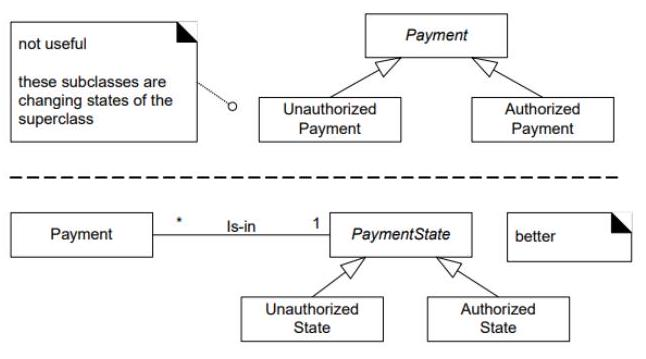
\includegraphics[width=\linewidth]{images/2024_12_29_0d1d7b5551ea1b4b41bdg-07(1)}

Abbildung 12: Zustände Domänenmodell(DM) Beispiel

\subsection*{4.2.5 Rollen (Manager etc.)}
Dasselbe Konzept (aber selten dieselbe Instanz) kann unterschiedliche Rollen einnehmen.\\
Dargestellt als Konzepte / Assoziationen

\subsection*{4.2.6 Assoziationsklasse}
\begin{center}
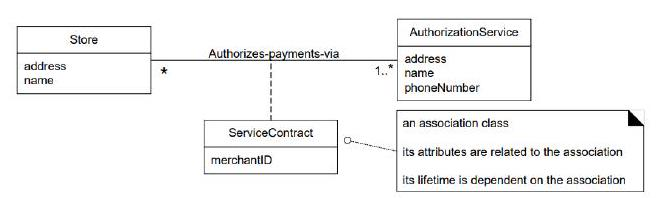
\includegraphics[width=\linewidth]{images/2024_12_29_0d1d7b5551ea1b4b41bdg-07}
\end{center}

Abbildung 13: Assoziationsklasse Beispiel

\subsection*{4.2.7 Masseinheiten / Zeitintervalle}
Oft Sinnvollerweise als Konzept modelliert